\section{Технический проект}
\subsection{Общая характеристика организации решения задачи}

Необходимо спроектировать и разработать программную систему, которая должна способствовать сокращению исходного кода программ без ущерба их функциональности за счёт возможностей метапрограммирования.

Для достижения этой цели было принято решение спроектировать язык программирования и создать программу для его интерпретации, удовлетворяющие описанным выше требованиям.

Главной задачей разработки интерпретатора языка программирования является создание программного обеспечения, которое способно интерпретировать и выполнить исходный программный код, написанный на определенном языке программирования, так, что результат выполнения соответствует правилам, описанным в спецификации интерпретируемого языка.

Для обеспечения конкурентоспособности интерпретатора, эта задача должна выполняться как можно более эффективно и быстро. Кроме того, он должен выполнять свою задачу в соответствии с главным принципом интерпретации -- код программы обрабатывается по одной инструкции или группе инструкций, выполняющихся сразу после анализа и обработки. 

Для реализации интерпретатора необходимо разработать следующие компоненты: лексический анализатор, объекты внутреннего представления, синтаксический анализатор, инструментарий выполнения команд языка и сборщик мусора.

\subsection{Обоснование выбора технологии проектирования}

Уже многие годы сфера ИТ предоставляет массу инструментов для разработки системного ПО, коим и является разработка интерпретатора.

\subsubsection{Описание используемых технологий и языков программирования}

В процессе разработки интерпретатора ДЯП используются язык программирования \quotes{C} и программные средства операционной системы семейства \quotes{GNU/Linux}. Используемые для создания программно-информационной системы средства отвечают современным практикам разработки и являются подходящими и достаточными для решения задач, выявленных при анализе предметной области.

\subsubsection{Язык программирования C}

Низкоуровневый язык программирования \quotes{C} (Си) -- один из первых языков программирования и, одновременно с этим, один из самых используемых до сих пор. Его появлению в начале 1970-х годов мир обязан инженеру Деннису Ритчи из американской компании \quotes{Bell Labs}, разрабатывавшим его как развитие языка \quotes{Би} для написания операционной системы \quotes{Unix} \cite{e7}. С тех пор Си стал одним из самых популярных языков для системного программирования.

Об успешности решений, принятых при его разработке, говорит впечатлительный список узнаваемых последователей, перенявших многие его идеи -- C++, C\#, Objective-C, Java, Python, PHP и другие обязаны Си своей структурой кода и базовым синтаксисом.

Узнаваемость и простота его синтаксиса, близость к аппаратной части ЭВМ, наличие компилятора почти для всех вычислительных устройств и операционных систем, обширная стандартная библиотека, а также ручное управление памятью убеждают в выборе языка С для системного программирования, коей и является разработка интерпретатора.

Ввиду того, что реализация стандартной библиотеки этого языка, libc, отличается для различных операционных систем, было принято решение выбрать целевой платформой для разработки интерпретатора одно семейство ОС -- \quotes{GNU/Linux}. В этих системах применяется реализация \quotes{GNU C Library} (glibc) \cite{e13}.


\subsection{Компоненты интерпретатора}

На рисунке \ref{interp_archit:image} в виде UML-диаграммы показаны компоненты, составляющие интерпретатор \cite{e26}.

\begin{figure}[ht]
	\center{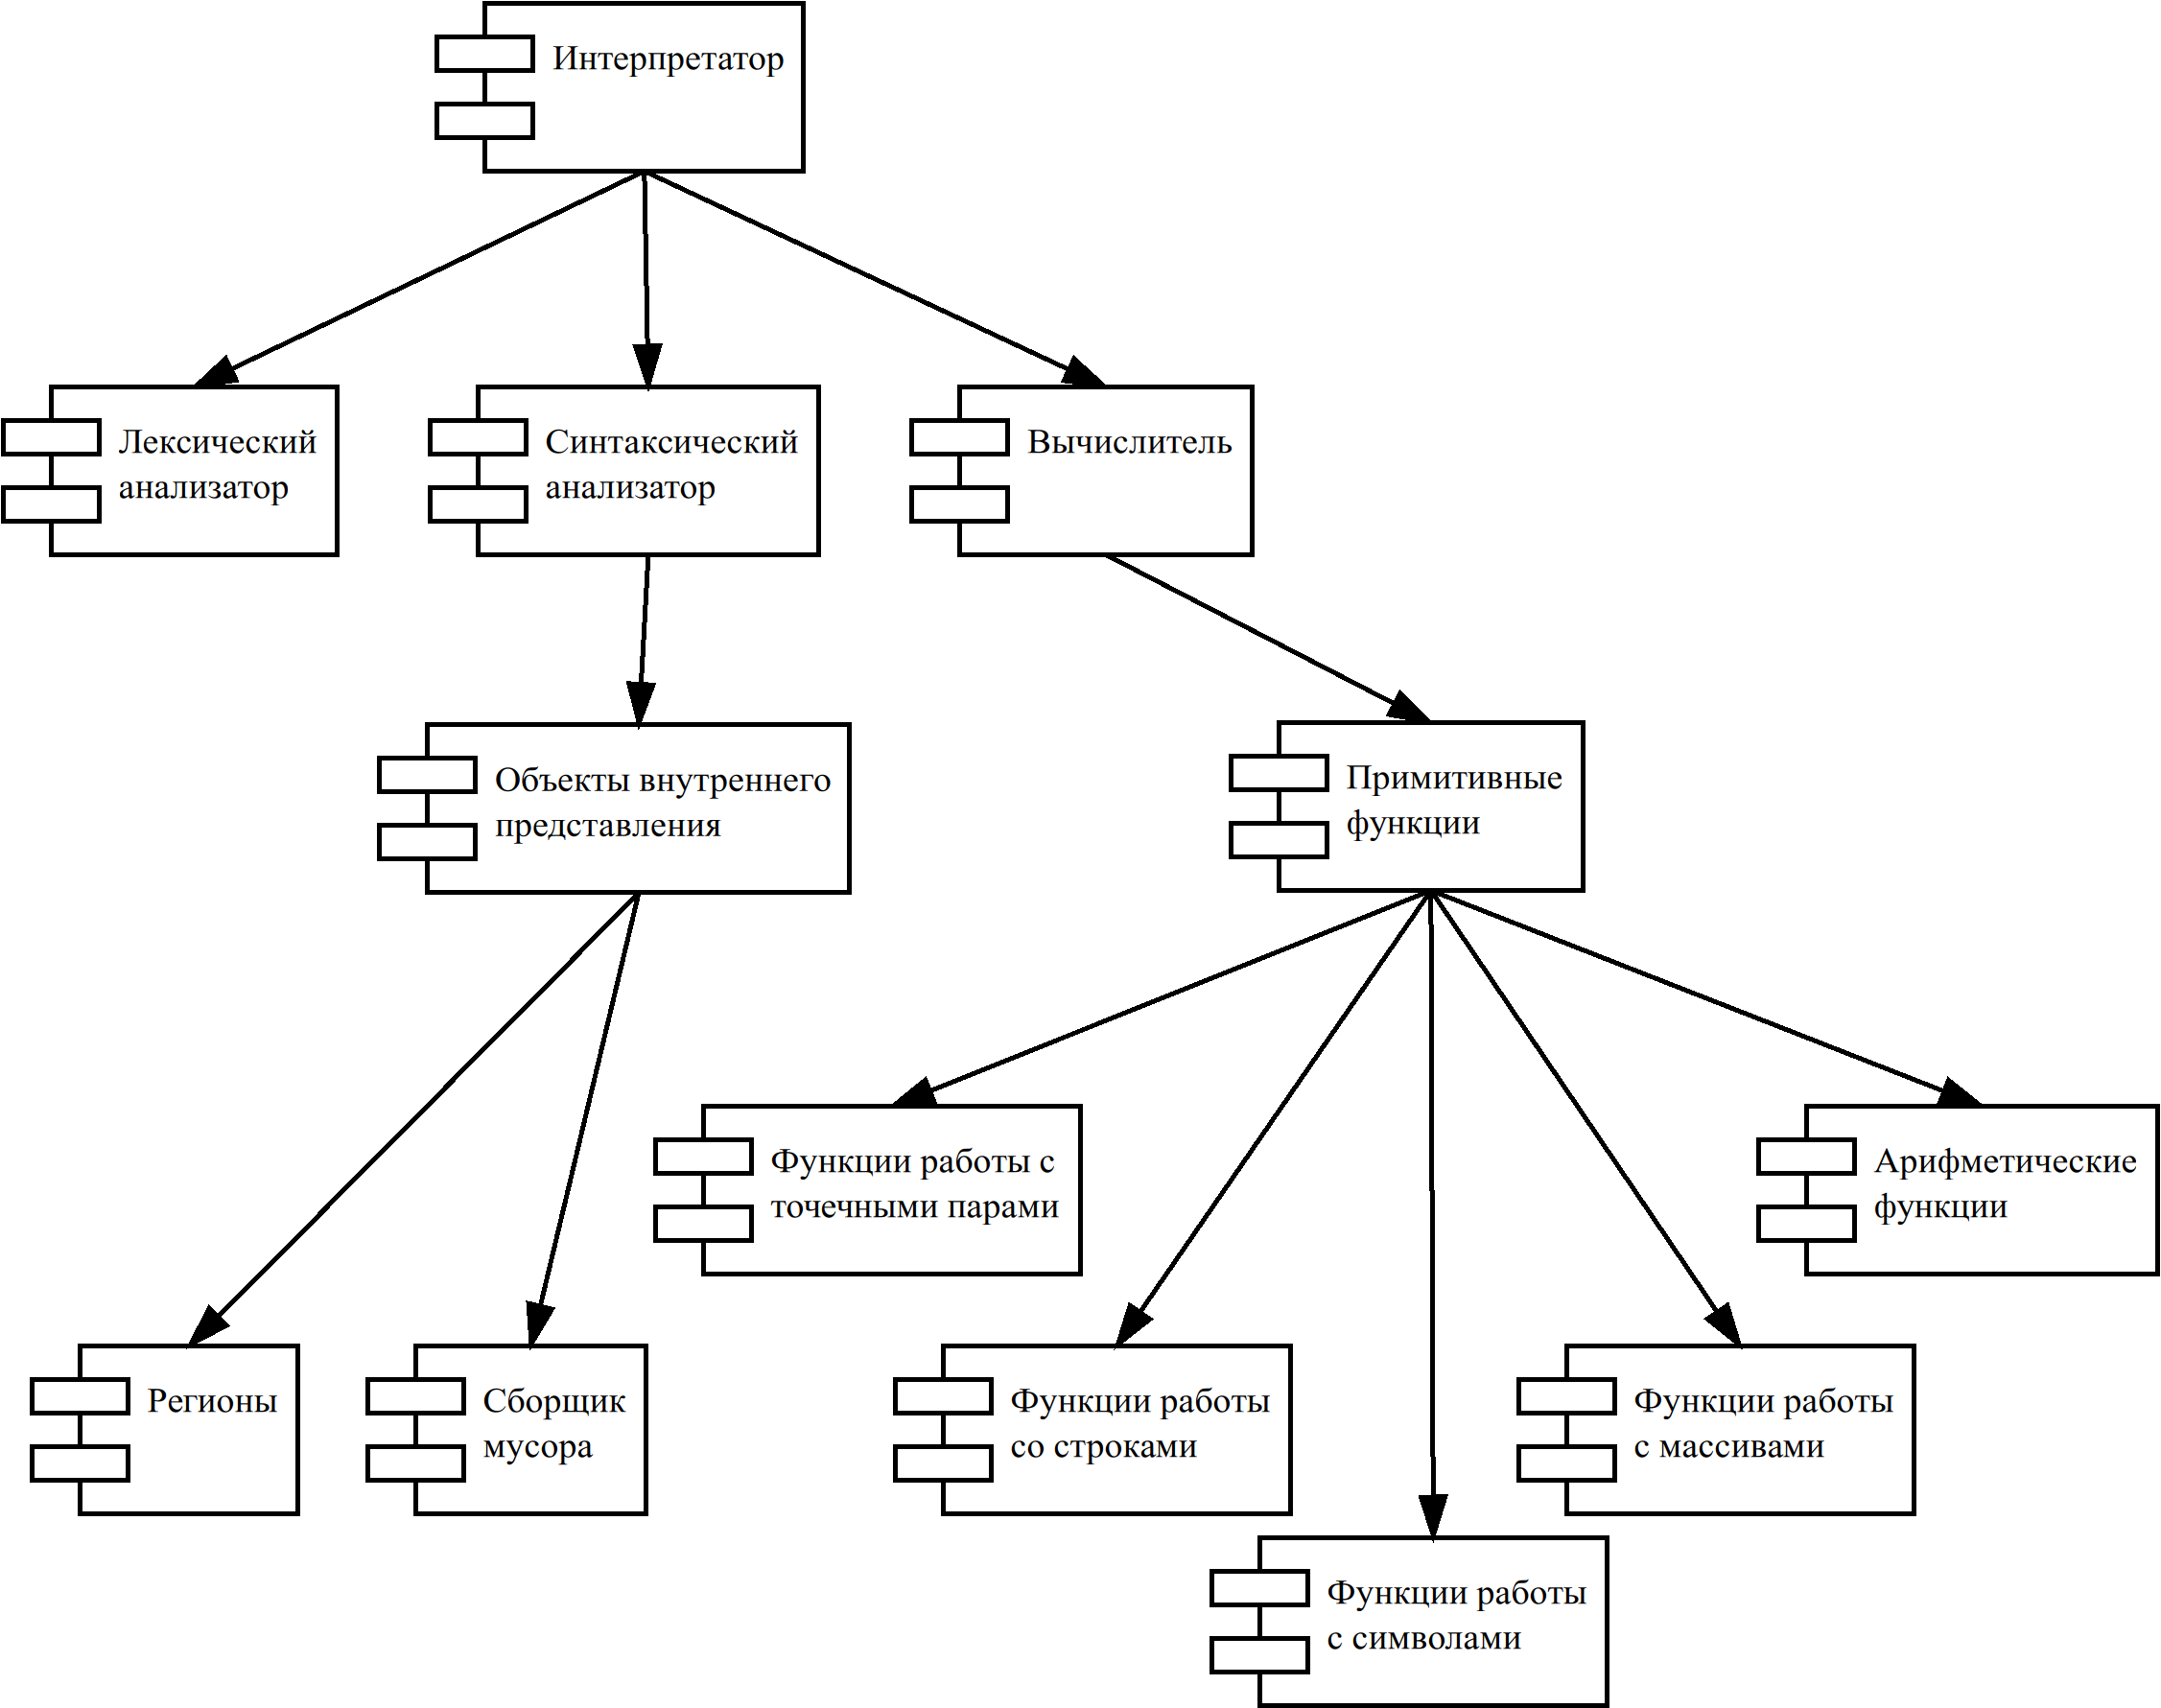
\includegraphics[width=1\linewidth]{interp_archit}}
	\caption{Диаграмма компонентов интерпретатора}
	\label{interp_archit:image}
\end{figure}

Таким образом, разработанный интерпретатор должен реализовывать следующие компоненты:
\begin{itemize}
	\item лексический анализатор -- для формирования токенов на основе текстового представления программы и выявления ошибок, связанных с использованием отсуствующих в алфавите языка символов или недопустимых в к использованию в некотором контексте символов (например, буква внутри числа: 124a6);
	\item синтаксический анализатор -- для формирования на основе токенов представления программы внутри интерпретатора и выявления синтаксических ошибок: отсутствие закрывающей скобки, отсутствие аргументов и тому подобные;
	\item вычислитель -- для выполнения инструкций, описанных в интерпретируемой программе;
	\item объекты внутреннего представления -- структуры, в которые будет преобразованы токены, для манипуляции данными из исходного кода в интерпретаторе;
	\item примитивные функции -- для реализации встроенных в язык функций, инструментов и конструкций, позволяющих производить манипуляции данными.
\end{itemize}

\subsubsection{Алгоритм взаимодействия компонентов}

На рисунке \ref{uml_coop:image} в виде UML-диаграммы взаимодействия показано как компоненты интерпретатора обмениваются данными.

\begin{figure}[H]
	\center{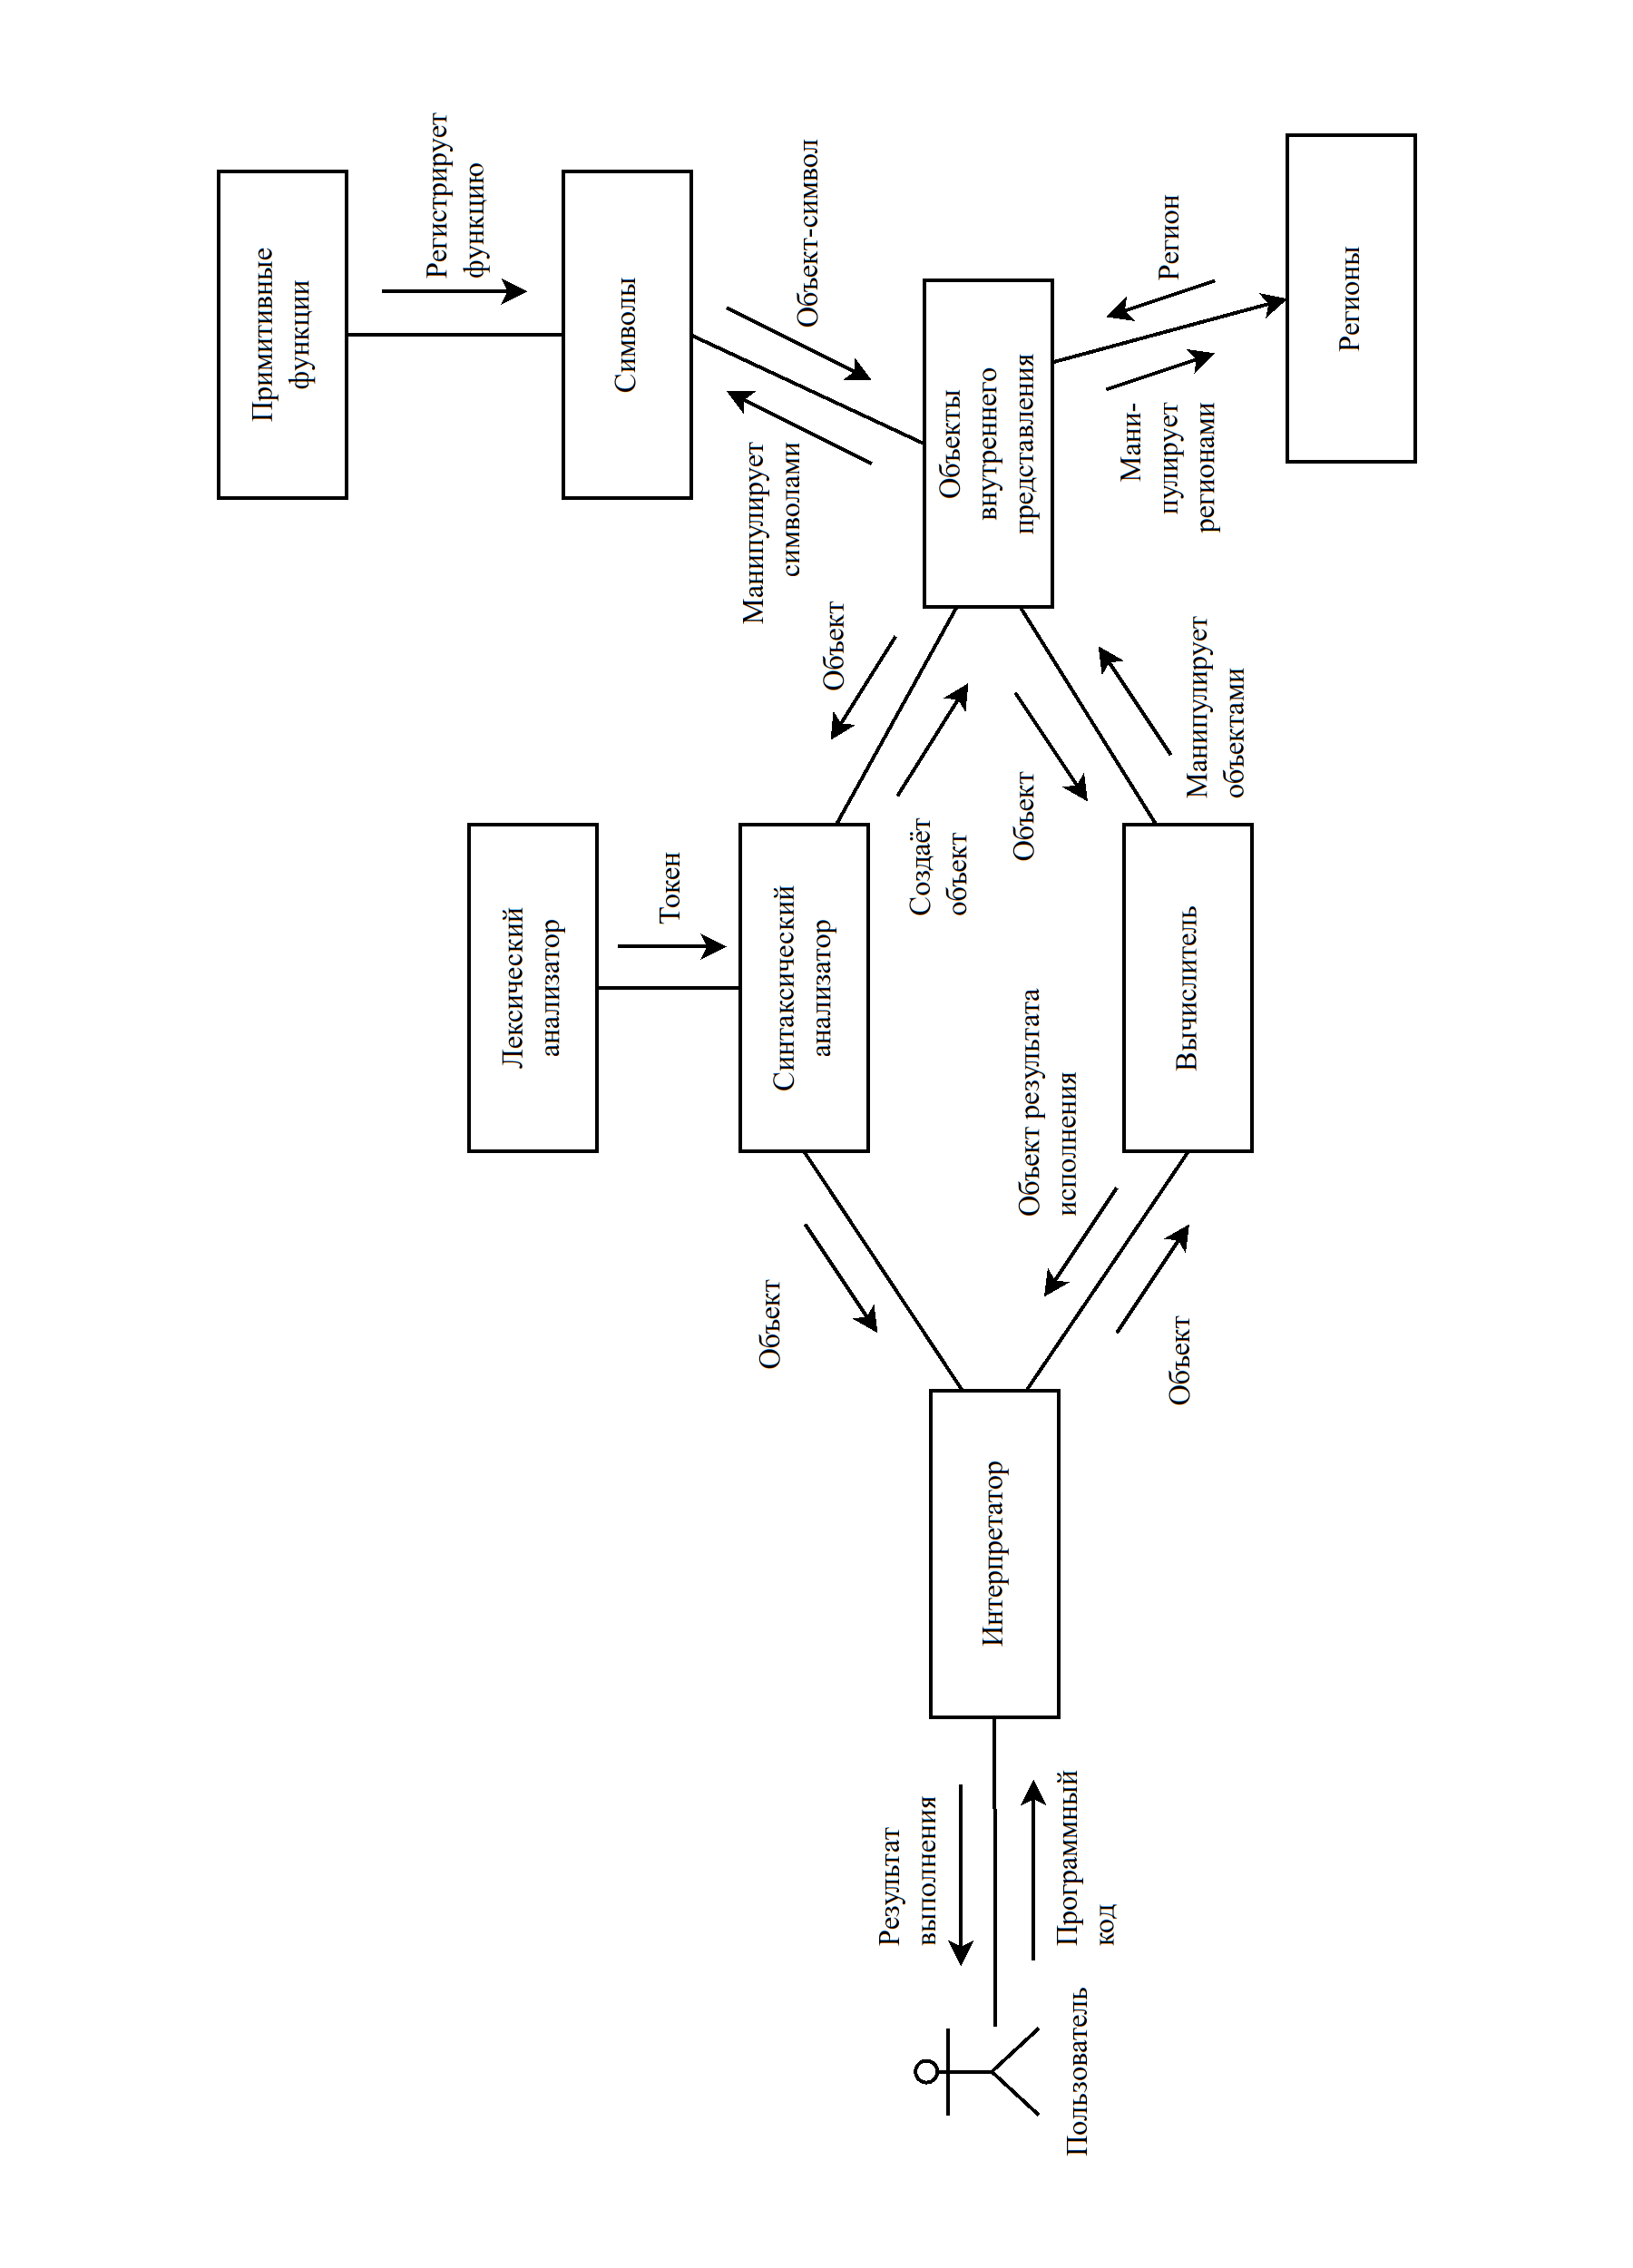
\includegraphics[width=1\linewidth]{uml_coop}}
	\caption{Диаграмма взаимодействия компонентов интерпретатора}
	\label{uml_coop:image}
\end{figure}

Пошаговый алгоритм взаимодействия компонентов, составляющих интерпретатор:

Шаг 1. Инициализируем вычислитель и регистрируем все примитивные функции ДЯП.

Шаг 2. Сохраняем текущее состояние программы, сохранив регистры процессора и стек с помощью setjmp. Если во время работы интерпретатора произойдёт ошибка -- вывести на экран сообщение об ошибке и перейти к шагу 8.

Шаг 3. Запускаем синтаксический анализатор.

Шаг 4. Синтаксический анализатор вызывает лексический анализатор.

Шаг 5. Лексический анализатор на основе символов из входного потока формирует лексему и возвращает её.

Шаг 6. Синтаксический анализатор на основе полученной лексемы формирует объект для внутреннего представления и возвращает его.

Шаг 7. Если был достигнут конец входного потока -- переходим к следующему шагу, иначе к шагу 12.

Шаг 8. Восстановить состояние программы к тому, что было сохранено на шаге 2, и перейти к шагу 13.

Шаг 9. Вычислитель производит вычисления с объектом, сформированным СА, в качестве аргумента и возвращает результат вычислений в виде объекта.

Шаг 10. Вывести возвращённый вычислителем объект на экран.

Шаг 11. Перейти к шагу 2.

Шаг 12. Сборщик мусора освобождает неиспользуемые объекты внутреннего представления. Перейти к шагу 2.

Шаг 13. Завершить работу интерпретатора.

\subsubsection{Лексический анализатор}
В разработанной программной системе лексический анализатор представляет собой компонент, в задачи которого входит считывание лексемы, проверка её на соответствие алфавиту языка и формирование токена.

Как только лексема была считана, она помещается в буфер размерностью в восемь символов.

Считанная лексема сравнивается со множеством зарезервированных под конструкции языка символов. При совпадении с каким-либо, формируется токен и ЛА возвращает его.


Сформированный токен представляет собой структуру с такими полями:
\begin{itemize}
	\item type -- тип токена;
	\item value -- поле для токенов числового типа, содержит значение числа;
	\item str -- поле для токенов строкового типа, значение строки.
\end{itemize}

Особым случаем является считывание строки. Как только обнаруживается символ кавычки, запускается функция, собирающая символы до тех пор, пока:
\begin{itemize}
	\item не встретит второй символ кавычки, чем будет закончено считывание строки, после чего ЛА вернёт сформированный токен;
	\item количество символов не превысит допустимую длину строки, что приведёт к ошибке;
	\item не будет достигнут конец входного потока, что также приведёт к ошибке.
\end{itemize}


Если лексема не является одной из зарезервированных, производится проверка на то, является она числом или символом.

Ввиду того, что имя символа, как и отрицательное число, может начинаться со знака минус, решается неоднозначность, связанная с восприятием ЛА следующих символов. Для этого считывается ещё один символ и, если он является числовым, дальнейшая запись определяется как число, иначе как символ.

Если имя символа состоит из допустимых знаков, то бишь из алфавита языка, формируется токен типа символ и возвращается как результат работы ЛА. В противном случае, выдаётся ошибка о некорректности символа.

\subsubsection{Синтаксический анализатор}
Синтаксический анализатор запрашивает у ЛА по одному токену, строит для них внутреннее представление и повторяет процесс, пока не будет сформировано одно s-выражение, затем происходит возврат выражения.

СА, как и ЛА, выполняет проверку на ошибки, но уже синтаксические. Он выявляет отсутствие аргументов у операторов цитирования и квазицитирования, неоконченость списков (отсутствие закрывающей скобки) и отсутствие списка после символа \quotes{\#} для создания массива.


\subsubsection{Объекты внутреннего представления}
Как уже было рассмотрено ранее, весь программный код, считываемый из потока ввода, ещё на этапе обработки лексическим анализатором преобразуется в особые структуры, а не хранится в виде текста, ввиду необходимости манипулирования предоставленной им информацией, что было бы проблематичным и неэффективным при текстовом хранении. После обработки синтаксическим анализатором, все данные, полученные из программного кода, принимают своё окончательное представление и при исполнении инструкций меняется уже не их представление, а содержимое.

В разрабатываемом интерпретаторе данные объектов хранятся в виде структур языка C, доступ к которым осуществляется через специальный указатель, называемый оболочкой объекта (object\_t, псевдоним типа long long размером 8 байт), содержащий в себе:
\begin{itemize}
	\item тип объекта (биты с 0 по 2): позволяет функциям узнать тип хранимых данных и верно их обработать;
	\item бит пометки (3 бит), необходимый для функционирования сборщика мусора. Используется только в точечных парах;
	\item данные объекта (биты с 4 по 64): малое число при числовом типе или указатель на экземпляр структуры данных, соответствующей одному из остальных типов.
\end{itemize}

Выделение и последующее чтение или изменение этих битов из оболочки происходит за счёт функций побитового сдвига \cite{e5}.

Тип объекта извлекается из оболочки с использованием макроса \quotes{TYPE}. Он возвращает числовое значение, соответствующее позиции типа в перечислении (enum) с индексами от нуля до пяти: NUMBER, BIGNUMBER, SYMBOL, PAIR, STRING, ARRAY.

Макросы \quotes{GET\_PAIR}, \quotes{GET\_BIGNUMBER}, \quotes{GET\_STRING}, \quotes{GET\_SYMBOL}, \quotes{GET\_ARRAY} позволяют получать из оболочки указатель на структуру, интерпретируемую в соответствии с выбранной функцией. Их работа основана на другом макросе -- \quotes{GET\_ADDR}, выделяющем адрес структуры в памяти из оболочки.

Оболочка объекта является результатом выполнения любого s-выражения и доступ из примитивных функций к структурам данных осуществляется только через неё. Всего было разработано пять структур, реализующих все доступные в языке типы, за исключением числового: большое число, пара, символ, строка, массив. Числовой же тип автоматически освобождается средствами языка \quotes{C}.

Далее под числовым типом будут подразумеваться как объекты типа \quotes{число}, так и \quotes{большое число}. При необходимости явно выделить последний, его наименование будет писаться полностью.

Структуры, представляющие данные объекта, по мере надобности распределяются из соответствующего для их типа пула -- массива фиксированного размера.

При необходимости создать экземпляр структуры, если список свободных структур этого типа, сформированный сборщиком мусора, пуст -- создаётся новый, иначе берётся из головы соответствующего типу списка свободных экземпляров.

Структуры этих пяти типов объектов представлены в таблицах \ref{strobjbignum:table} -- \ref{strobjsym:table}.

\begin{xltabular}{\textwidth}{|l|l|p{5.7cm}|X|}
	\caption{Структура \quotes{bignumber\_t} для объекта типа \quotes{большое число}\label{strobjbignum:table}}\\ \hline
	\centrow Имя & \centrow Тип & \centrow Описание & \centrow Возможные значения \\ \hline
	%\thead{1} & \thead{2} & \centrow 3 & \centrow 4 \\ \hline
	%\endfirsthead
	%\continuecaption{Продолжение таблицы \ref{strobjbignum:table}}
	%\thead{1} & \thead{2} & \centrow 3 & \centrow 4 \\ \hline
	\finishhead
	value & int & Числовое значение & Нет ограничений \\ \hline 
	next & object\_t* & Указатель для сборщика мусора на следующий свободный объект-пару & Если NULL — данная пара является последней в списке свободных или список пуст, иначе содержит указатель на следующий свободный объект-пару. \\ \hline 
	free & int & Свободна ли пара для перезаписи  & Если 1 — пара в списке свободных пар, иначе занята
\end{xltabular}

\begin{xltabular}{\textwidth}{|l|l|p{5.7cm}|X|}
	\caption{Структура \quotes{pair\_t} для объекта-пары\label{strobjpair:table}}\\ \hline
	\centrow Имя & \centrow Тип & \centrow Описание & \centrow Возможные значения \\ \hline
	\thead{1} & \thead{2} & \centrow 3 & \centrow 4 \\ \hline
	\endfirsthead
	\continuecaption{Продолжение таблицы \ref{strobjpair:table}}
	\thead{1} & \thead{2} & \centrow 3 & \centrow 4 \\ \hline
	\finishhead
	left & object\_t* & Указатель на левый элемент пары & Указатель на объект или NULL \\ \hline 
	right & object\_t* & Указатель на правый элемент пары & Указатель на объект или NULL \\ \hline 
	next & object\_t* & Указатель для сборщика мусора на следующий свободный объект-пару & Если NULL — данная пара является последней в списке свободных или список пуст, иначе содержит указатель на следующий свободный объект-пару. \\ \hline 
	free & int & Свободна ли пара для перезаписи  & Если 1 — пара в списке свободных пар, иначе занята
\end{xltabular}

\begin{xltabular}{\textwidth}{|l|l|p{5.7cm}|X|}
	\caption{Структура \quotes{string\_t} для объекта-строки\label{strobjstr:table}}\\ \hline
	\centrow Имя & \centrow Тип & \centrow Описание & \centrow Возможные значения \\ \hline
	%\thead{1} & \thead{2} & \centrow 3 & \centrow 4 \\ \hline
	%\endfirsthead
	%\continuecaption{Продолжение таблицы \ref{strobjstr:table}}
	%\thead{1} & \thead{2} & \centrow 3 & \centrow 4 \\ \hline
	\finishhead
	data & char* & Данные строки & Нет ограничений \\ \hline 
	length & int & Длина строки & Натуральное число, соответствующее количеству символов в строке \\ \hline 
	next & string\_t* & Указатель для сборщика мусора на следующую свободную строковый объект & Если NULL — данная строка является последней в списке свободных или список пуст, иначе содержит указатель на следующую свободную объект-пару. \\ \hline 
	free & int & Свободна ли строка для перезаписи & Если 1 — строка в списке свободных строк, иначе занята
\end{xltabular}


\begin{xltabular}{\textwidth}{|l|l|p{5.7cm}|X|}
	\caption{Структура \quotes{array\_t} для объекта-массива\label{strobjarr:table}}\\ \hline
	\centrow Имя & \centrow Тип & \centrow Описание & \centrow Возможные значения \\ \hline
	\thead{1} & \thead{2} & \centrow 3 & \centrow 4 \\ \hline
	\endfirsthead
	\continuecaption{Продолжение таблицы \ref{strobjarr:table}}
	\thead{1} & \thead{2} & \centrow 3 & \centrow 4 \\ \hline
	\finishhead
	data & object\_t** & Данные массива & Нет ограничений \\ \hline 
	length & int & Количество элементов массива & Натуральное число, соответствующее количеству элементов массива \\ \hline 
	next & array\_t* & Указатель для сборщика мусора на следующий свободный массив & Если NULL — данный объект-массив является последним в списке свободных или список пуст, иначе содержит указатель на следующий свободный объект-массив. \\ \hline 
	free & int & Свободен ли массив для перезаписи & Если 1 — массив в списке свободных массивов, иначе занят
\end{xltabular}

\begin{xltabular}{\textwidth}{|l|l|p{5.7cm}|X|}
	\caption{Структура \quotes{symbol\_t} для объекта-символа\label{strobjsym:table}}\\ \hline
	\centrow Имя & \centrow Тип & \centrow Описание & \centrow Возможные значения \\ \hline
	\thead{1} & \thead{2} & \centrow 3 & \centrow 4 \\ \hline
	\endfirsthead
	\continuecaption{Продолжение таблицы \ref{strobjsym:table}}
	\thead{1} & \thead{2} & \centrow 3 & \centrow 4 \\ \hline
	\finishhead
	str & char[] & Имя символа & NUMBER \\ \hline 
	next & symbol\_t* & Указатель на следующий за данным символ в хеш-таблице & Нет ограничений \\ \hline 
	value & object\_t * & Указатель на объект, связанный с символом & Если NULL — данный объект является последним в списке свободных или список пуст, иначе содержит указатель на следующий свободный объект. \\ \hline 
	lambda & object\_t* & Указатель на объект лямбда-выражения, связанный с символом & Если 1 — связан, 0 — не связан. \\ \hline
	macro & object\_t & Указатель на объект макроса, связанный с символом & Если 1 — связан, 0 — не связан. \\ \hline
	func & func\_t & Указатель на примитивную функцию, связанную с символом. & Нет ограничений
\end{xltabular}

\quotes{func\_t} -- это указатель на функцию, которая принимает \quotes{object\_t} в качестве аргумента и возвращает \quotes{object\_t}.

\subsubsection{Вычислитель}

Вычислитель получает на вход два значения:
\begin{itemize}
\item obj -- объект, представляющий s-выражение, которое необходимо выполнить;
\item env -- окружение, в котором s-выражение obj будет выполняться.
\end{itemize}

Ниже приведено пошаговое представление алгоритма работы вычислителя, где некоторые шаги имеют подшаги, которые также надо пройти, если условие шага верхнего уровня выполняется:

Шаг 1. Если объект obj равен NULLOBJ, вернуть NULLOBJ, окончив этим выполнение алгоритма.

Шаг 2. Иначе, если тип obj равен NUMBER, BIGNUMBER, STRING или ARRAY -- вернуть obj, окончив этим выполнение алгоритма.

Шаг 3. Иначе, если тип obj равен SYMBOL.

Подшаг 3.1. Если в env есть объект, содержащий указатель на искомый символ, вернуть этот объект, окончив этим выполнение алгоритма.

Подшаг 3.2. Иначе проверить наличие символа, соответствующего имени искомого, в хеш-таблице. Если символ найден и ссылается на объект, содержащий его, вернуть данный объект, окончив этим выполнение алгоритма.

Подшаг 3.3. Иначе вызвать функцию error с описанием ошибки об отсутствии символа, которое будет выведено на экран, окончив этим выполнение алгоритма.

Шаг 4. Иначе, если тип obj равен PAIR.

Подшаг 4.1. Если первый элемент цепи obj является цепью.

Подшаг 4.1.1. Если первый элемент цепи obj имеет особенности, указывающие на то, что он является лямбда-выражением -- выполнить это лямбда-выражение в окружении env и вернуть результат, окончив этим выполнение алгоритма.

Подшаг 4.1.2. Иначе вызвать функцию error с описанием ошибки в структуре лямбда-выражения, которое будет выведено на экран, окончив этим выполнение алгоритма.

Подшаг 4.2. Ввести переменную s. Найти (или создать при отсутствии), символ в хеш-таблице, имя которого соответствует имени искомого, и задать значением для s этот символ; Ввести переменную args.

Подшаг 4.3. Если первый элемент цепи obj имеет особенности, позволяющие определить его как специальную форму, задать для args значение хвоста цепи obj.

Подшаг 4.4. Иначе рекурсивно вычислить в окружении env список аргументов из хвоста цепи obj.

Подшаг 4.5. Если символ s содержит указатель на функцию -- выполнить её с аргументами args в окружении env и вернуть вычисленное значение, окончив этим выполнение алгоритма.

Подшаг 4.6. Иначе, если символ s содержит указатель на функцию примитивного типа -- выполнить её с аргументами args и вернуть вычисленное значение, окончив этим выполнение алгоритма.

Подшаг 4.7. Иначе, если символ s содержит указатель на макрос -- вычислить макро-подстановку с аргументами args в окружении env и вернуть вычисленное значение, окончив этим выполнение алгоритма.

Подшаг 4.8. Иначе вызвать функцию error с описанием ошибки о том, что функцию не удалось найти, окончив этим выполнение алгоритма.

Шаг 5. Иначе вызвать функцию error с описанием ошибки о том, что вычислитель не может определить тип переданного ему объекта. Конец алгоритма.

\subsubsection{Сборщик мусора}
Спроектированный в рамках этой работы сборщик мусора работает в две фазы по алгоритму пометки и очистки и осуществляет сборку по следующему принципу:

\begin{enumerate}
	\item Фаза пометки.
	Обходим все символы в таблице символов и выполняем пометку объектов, на которые они указывают. Пометка реализуется через третий бит оболочки объекта. Если помечается объект-пара, то левый и правый объекты этой пары пометятся рекурсивно;
	
	\item Фаза очистки.
	Обходим все выделенные объекты и пары. Если есть пометка -- снимаем её, иначе рекурсивно освобождаем объект, задавая значением для поля \quotes{free} число 1. Для \quotes{next} указываем следующий свободный объект, а только что освобождённый добавляется в начало соответствующего списка свободных объектов.
	
\end{enumerate}

Объекты освобождаются в конце вычисления выражения верхнего уровня. Объекты типа \quotes{символ} и \quotes{число (маленькое)} сборщиком не затрагиваются.

Пометка производится в бит пометки, под который выделена часть в одном из полей экземпляра структуры. Для разных структур оно отличается:
\begin{itemize}
	\item большие числа -- старший бит поля free (int, 4 байта);
	\item точечные пары -- четвёртый бит поля left (long long, 8 байт);
	\item строки и массивы -- старший бит поля length (int, 4 байта).
\end{itemize}

Таким образом, в случае больших чисел, массивов и строк запись производится непосредственно в один их элементов структуры объекта, а в случае пар -- в оболочку объекта \quotes{object\_t}.

Пометка реализуется функцией \quotes{mark\_object}, принимающей в качестве аргумента оболочку объекта и производит пометку данных, на которые она ссылается. В случае с парами, пометка производится рекурсивно.

Освобождение непомеченных объектов выполняет функция \quotes{sweep}.

Сборщиком мусора формируются списки объектов разных типов, которые были освобождены для дальнейшей перезаписи: \quotes{free\_bignumbers}, \quotes{free\_pairs}, \quotes{free\_strings} и \quotes{free\_arrays}. В программной реализации они представляют собой указатели на некоторый объект, освободившийся последним, через поле \quotes{next} которого можно продвигаться по списку дальше, к следующим свободным объектам, пока не будет достигнуто значение NULL, означающее конец списка.

Если такой список не пуст, то есть не равен \quotes{NULL}, при необходимости создать объект, вместо этого он будет взят из головы списка и его поля будут перезаписаны, после чего голова будет сдвинута на значение вперёд по полю \quotes{next}.



\subsubsection{Примитивные функции}

Было реализовано множество функций, встроенных в разрабатываемый язык.

\paragraph{Арифметические функции}

Разработанные арифметические функции позволяют выполнять базовые арифметические операции вроде суммирования и деления, а также побитовые, эквивалентности и сравнения. Перечень таких функций, их описания и примеры использования представлены в таблице \ref{funcprimarith:table}.

Также там содержатся перечни типов обрабатываемых функцией аргументов. Перечисление происходит через запятую, если функция принимает сразу несколько аргументов. Если же необходимо указать что для одного аргумента функция может принимать объекты определённых нескольких типов, они записываются через "или".

\begin{xltabular}{\textwidth}{|p{3.6cm}|p{2cm}|p{6cm}|X|}
	\caption{Перечень функций арифметического модуля\label{funcprimarith:table}}\\ \hline
	\centrow Имя & \centrow Аргу- \linebreak менты & \centrow Описание & \centrow Пример \\ \hline
	\thead{1} & \thead{2} & \centrow 3 & \centrow 4 \\ \hline
	\endfirsthead
	\continuecaption{Продолжение таблицы \ref{funcprimarith:table}}
	\thead{1} & \thead{2} & \centrow 3 & \centrow 4 \\ \hline
	\finishhead
	Суммирование & Числа & Возвращает сумму чисел списка & < (+ 1 2 3) \linebreak > 6 \\ \hline 
	Вычитание & Числа & Возвращает разность чисел списка & < (- 5 2 1) \linebreak > 2 \\ \hline 
	Произведение & Числа & Возвращает произведение чисел списка & < (* 2 1 2) \linebreak 4 \\ \hline 
	Деление & Числа & Возвращает результат от деления чисел списка & < (/ 8 2) \linebreak 4 \\ \hline 
	Больше чем & Числа & Возвращает результат сравнения на большее из двух чисел списка. Если левое больше правого -- T, иначе NIL & < (> 2 1) \linebreak > T \\ \hline 
	Меньше чем & Числа & Возвращает результат сравнения на меньшее из двух чисел списка. Если левое меньше правого -- T, иначе NIL & < (< 2 1) \linebreak > NIL \\ \hline 
	Разность чисел & Числа & Возвращает результат сравнения на меньшее из двух чисел списка. Если числа равны -- T, иначе NIL & < (= 2 1) \linebreak > NIL \\ \hline 
	Эквивалентность объектов по значению & Любые & Возвращает результат сравнения значений двух объектов списка. Если значения идентичны -- T, иначе NIL & < (equal 2 2) \linebreak > T \\ \hline 
	Побитовое И & Числа & Возвращает результат побитового умножения чисел списка & < (\& 1 1 0) \linebreak > 0 \\ \hline 
	Побитовое ИЛИ & Числа & Возвращает результат побитового сложения чисел списка & < (bitor 1 1 0) \linebreak > 0 \\ \hline 
	Побитовый сдвиг влево & Числа & Первый аргумент -- число, на которое будет применён сдвиг, второй -- число бит сдвига. Возвращает результат побитового сдвига влево числа & < (<< 1 2) \linebreak > 8 \\ \hline 
	Побитовый сдвиг вправо & Числа & Первый аргумент -- число, на которое будет применён сдвиг, второй -- число бит сдвига. Возвращает результат побитового сдвига вправо числа & < (>> 0xF0 8) \linebreak > 15
\end{xltabular}

\paragraph{Функции вычислителя}

Вычислитель содержит в своём модуле все функции, отвечающие за:
\begin{itemize}
	\item объявление функций, переменных, макросов и их вычисление нестандартными способами;
	\item логические операторы;
	\item создание списков;
	\item цитирование и квазицитирование;
	\item проверка объектов на атомарность и эквивалентность атомов.
\end{itemize}

Полный перечень функций представлен в таблице \ref{funcprimeval:table}.

\begin{xltabular}{\textwidth}{|p{3.6cm}|p{1.8cm}|p{6cm}|X|}
	\caption{Перечень функций вычислительного модуля\label{funcprimeval:table}}\\ \hline
	\centrow Имя & \centrow Аргу- \linebreak менты & \centrow Описание & \centrow Пример \\ \hline
	\thead{1} & \thead{2} & \centrow 3 & \centrow 4 \\ \hline
	\endfirsthead
	\continuecaption{Продолжение таблицы \ref{funcprimeval:table}}
	\thead{1} & \thead{2} & \centrow 3 & \centrow 4 \\ \hline
	\finishhead
	Проверка на атом & Любой & Если объект является атомом -- возвращает T, иначе NIL & < (atom 'a) \linebreak > T \\ \hline 
	Эквивалентность атомов & Любые & Если два атома равны -- возвращает T, иначе NIL & < (eq 'a 'a) \linebreak > T \\ \hline 
	Цитирование & Любой & Возвращает аргумент без вычисления & < (quote (+ 1 2)) \linebreak > (+ 1 2) \\ \hline 
	Квазицитирова-\linebreak ние & Любой & Возвращает аргумент с частичными вычислениями & < (setq b 1) \linebreak < (backquote (+ ,b 2 3)) \linebreak > (+ 1 2 3) \\ \hline 
	Условие & Списки & Аргументы вычисляются до тех пор, пока не будет достигнут результат вычисления T. Каждый аргумент -- список, где первый элемент -- проверяемое выражение, а второй -- результат, который будет возвращен при истинности выражения & < (cond ((eq 'a 'b) 1) (t 2)) \linebreak > 2 \\ \hline 
	Объявление функции & Символ, списки & Объявляет новую функцию с именем, соответствующим первому аргументу, списку параметров -- второму аргументу и телу функции -- третьему & < (defun pl (x) (+ 1 x)) \linebreak < (pl 2) \linebreak > 3 \\ \hline 
	Применение функции к аргументам & Символ или лямбда-выра- \linebreak жение, любые & Эта функция применяет значение первого аргумента как функцию к остальным аргументам и возвращает результат применения & < (funcall '+ 1 2) \linebreak > 3 \\ \hline 
	Объявление макроса & Символ, списки & Объявляет новый макрос с именем, соответствующим первому аргументу, списку параметров -- второму аргументу и телу макроса -- третьему & < (defmacro db (x) `(* 2 ,x)) \linebreak < (db 3) \linebreak > 6 \\ \hline 
	Макроподста-\linebreak новка & Список & Возвращает результат макроподстановки для переданного в качестве аргумента квотированного вызова макроса & < (defmacro db (x) `(* 2 ,x)) \linebreak < (macroexpand '(db 3)) \linebreak > (* 2 3) \\ \hline 
	Последова-\linebreak тельное выполнение & Любые & Последовательно вычисляет все s-выражения, переданные в качестве аргументов, и возвращает результат последнего вычисленного & < (progn  (+ 1 2) 5) \linebreak > 5 \\ \hline 
	Объявление переменной & Символ, любой & Объявляет переменную с именем, переданным в качестве первого аргумента, и значением -- второго. & < (setq val 3) \linebreak > 3 \\ \hline 
	Логическое ИЛИ & Списки & Возвращает T после нахождения первого истинного условия. Если истинных нет -- вернёт NIL. Должно быть хотя бы одно условие & < (or (= 1 2)) \linebreak > NIL \\ \hline 
	Логическое И & Списки & Возвращает NIL после нахождения первого ложного условия. Если ложных нет -- вернёт T. Должно быть хотя бы одно условие & < (and (> 2 1) (< 1 2)) \linebreak > T \\ \hline 
	Создание списка & Любые & Возвращает список, сформированный из переданных аргументов & < (list 1 'x '(12 3)) \linebreak > (1 X (12 3)) \\ \hline 
	Вычисление s-выражения & Любой & Вычисляет s-выражение и возвращает результат его вычисления & < (eval '(/ 4 2)) \linebreak > 2 \\ \hline 
\end{xltabular}

\paragraph{Функции модуля работы с массивами}

Этот модуль функций включает инструменты для создания массива, получения и установки значения.

Полный перечень функций представлен в таблице \ref{funcprimarr:table}.

\begin{xltabular}{\textwidth}{|p{3.6cm}|p{1.8cm}|p{6cm}|X|}
	\caption{Перечень функций модуля работы с массивами\label{funcprimarr:table}}\\ \hline
	\centrow Имя & \centrow Аргу- \linebreak менты & \centrow Описание & \centrow Пример \\ \hline
	%\thead{1} & \thead{2} & \centrow 3 & \centrow 4 \\ \hline
	%\endfirsthead
	%\continuecaption{Продолжение таблицы \ref{funcprimarr:table}}
	%\thead{1} & \thead{2} & \centrow 3 & \centrow 4 \\ \hline
	\finishhead
	Создание пустого массива & Число & Создает пустой массив заданной аргументом длины и возвращает его & < (make-array 3) \linebreak > \#(NIL NIL NIL) \\ \hline 
	Размер массива & Массив & Возвращает размер массива & < (array-size \#(1 2)) \linebreak > 2 \\ \hline
	Задать значение элементу & Массив, число, любой & Задает значение элементу массива с некоторым индексом и возвращает массив. Аргументы: массив, индекс, значение & < (seta \#(1 2) 0 10)) \linebreak > \#(10 2) \\ \hline 
	Чтение элемента & Массив, число & Возвращает значение элемента массива по некоторому индексу. Аргументы: массив, индекс & < (aref \#(4 2) 1) \linebreak > 2 \\ \hline 
	
\end{xltabular}

\paragraph{Функции модуля работы с точечными парами}

Этот модуль реализует инструменты для работы со списками и точечными парами.

Полный перечень функций представлен в таблице \ref{funcprimpair:table}.

\begin{xltabular}{\textwidth}{|p{3.6cm}|p{1.8cm}|p{6cm}|X|}
	\caption{Перечень функций модуля работы с точечными парами\label{funcprimpair:table}}\\ \hline
	\centrow Имя & \centrow Аргу- \linebreak менты & \centrow Описание & \centrow Пример \\ \hline
	%\thead{1} & \thead{2} & \centrow 3 & \centrow 4 \\ \hline
	%\endfirsthead
	%\continuecaption{Продолжение таблицы \ref{funcprimpair:table}}
	%\thead{1} & \thead{2} & \centrow 3 & \centrow 4 \\ \hline
	\finishhead
	Первый элемент & Список & Возвращает первый элемент переданного аргументом списка & < (car '(a b)) \linebreak > A \\ \hline 
	Исключение первого элемента & Список & Возвращает переданный аргументом список без первого элемента & < (cdr '(a b c)) \linebreak > B C \\ \hline 
	Создание пары & Список & Создаёт точечную пару, где левая часть -- первый элемент переданного аргументом списка, правая -- второй. & < (cons 'a 'b) \linebreak > (A . B) \\ \hline 
	Заменить левую часть пары & Пара, любой & Заменяет левую часть пары, переданной первым аргументом, значением второго аргумента и возвращает получившуюся пару & < (rplaca '(a . b) 'd) \linebreak > (D . B) \\ \hline 
	Заменить правую часть пары & Пара, любой & Заменяет правую часть пары, переданной первым аргументом, значением второго аргумента и возвращает получившуюся пару & < (rplacd '(a . b) 'd) \linebreak > (A . D)
	
\end{xltabular}

\paragraph{Функции модуля работы со строками}

Этот модуль реализует инструменты для работы непосредственно со строками и строковыми преобразованиями, а также с именами символов

Полный перечень функций представлен в таблице \ref{funcprimstr:table}.

\begin{xltabular}{\textwidth}{|p{3.6cm}|p{1.8cm}|p{6cm}|X|}
	\caption{Перечень функций модуля работы со строками\label{funcprimstr:table}}\\ \hline
	\centrow Имя & \centrow Аргу- \linebreak менты & \centrow Описание & \centrow Пример \\ \hline
	\thead{1} & \thead{2} & \centrow 3 & \centrow 4 \\ \hline
	\endfirsthead
	\continuecaption{Продолжение таблицы \ref{funcprimstr:table}}
	\thead{1} & \thead{2} & \centrow 3 & \centrow 4 \\ \hline
	\finishhead
	Создание символа & Строка & Создаёт символ с именем, соответствующим первому аргументу, и возвращает созданный символ & < (intern "A") \linebreak > A \\ \hline 
	Объединение двух строк & Строка, строка & Возвращает объединение двух строк, переданных аргументами & < (concat "a" "\_") \linebreak > "a\_" \\ \hline 
	Получение имени символа & Символ & Возвращает имя символа, переданного в качестве аргумента & < (symbol-name 'sym) \linebreak > SYM \\ \hline 
	Получение длины строки & Строка & Возвращает длину строки, переданной в качестве аргумента & < (string-size "123") \linebreak > 3 \\ \hline 
	Получение символа из строки & Строка, число & Возвращает код символа из строки по некоторому индексу & < (char "123" 2) \linebreak > 51 \\ \hline 
	Получение подстроки & Строка, число, число & Возвращает подстроку из строки, начиная с начального индекса и по конечный индекс, не включая последний. Аргументы: строка начальный\_индекс конечный\_индекс & < (subseq "123" 0 2) \linebreak > "12" \\ \hline 
	Число в строку & Число & Возвращает строку, содержащую число, переданное в качестве аргумента & < (inttostr 12) \linebreak > "12" \\ \hline 
	Код символа в строку & Число & Возвращает символ в строковом представлении на основе кода символа, переданного в качестве аргумента & < (code-char 51) \linebreak > 3
	
\end{xltabular}

Также была разработана функция для проверки объекта на принадлежность к символам -- \quotes{symbolp}. Если переданный ей объект является символом, она возвращает T, иначе NIL. Пример использования:
\begin{lstlisting}[language=Lisp, frame=none]
< (symbolp 'a)
> T
\end{lstlisting}


\subsection{Символы}

Ввиду того, что объекты-символы необходимо получать по имени и делать это часто, для их хранения был выбран способ хеш-таблицы. Хранение в массиве и поиск символов в нём с помощью перебора будет занимать всё больше времени по мере роста количества элементов. С хеш-таблицей \cite{e16} же перебор не требуется, потому время не возрастает. Этот способ основан на вычислении специального целочисленного значения, хеша, на основе имени символа. Хеш для каждого уникального имени так же будет уникальным. Таким образом, можно реализовать систему, где значение хеша будет являться индексом элемента в массиве и выполнять запись и чтение с помощью него.

Для реализации этого мезанизма был создан массив со значениями типа symbol\_t. Разработанная хеш-функция позволяет генерировать 257659 индексов. Для отслеживания количества созданных символов имеется переменная last\_symbol с изначальным значением \quotes{0}, которое повышается на единицу при создании нового символа. Такое отслеживание необходимо для контроля за тем, когда максимально возможное количество символов в массиве будет достигнуто, а также получения сборщиком мусора информации о том, сколько символов ему необходимо обходить на фазе пометки.

Поля и функции, разработанные для реализации таблицы символов, добавления в неё элементов и поиска представлены в таблицах \ref{module_str_sym_fields:table} и \ref{module_str_sym_funcs:table} соответственно.

\begin{xltabular}{\textwidth}{|l|p{3.5cm}|X|}
	\caption{Спецификация полей модуля \quotes{symbols.c}\label{module_str_sym_fields:table}}\\ \hline
	\centrow Имя & \centrow Тип & \centrow Описание \\ \hline
	%\thead{1} & \thead{2} & \centrow 3 \\ \hline
	%\endfirsthead
	%\continuecaption{Продолжение таблицы \ref{module_str_sym_fields:table}}
	%\thead{1} & \thead{2} & \centrow 3 \\ \hline
	\finishhead
	HASH\_SIZE & Символическая константа & Задаёт размер хеш-таблицы \\ \hline
	MAX\_SYMBOL\_SIZE & Символическая константа & Задаёт максимальную длину имени символа \\ \hline
	hash\_table & symbol\_t* [] & Хеш-таблица размером \quotes{HASH\_SIZE} для хранения символов
\end{xltabular}

\begin{xltabular}{\textwidth}{|l|p{4cm}|X|}
	\caption{Спецификация методов модуля \quotes{symbols.c}\label{module_str_sym_funcs:table}}\\ \hline
	\centrow Имя & \centrow Тип & \centrow Описание \\ \hline
	\thead{1} & \thead{2} & \centrow 3 \\ \hline
	\endfirsthead
	\continuecaption{Продолжение таблицы \ref{module_str_sym_funcs:table}}
	\thead{1} & \thead{2} & \centrow 3 \\ \hline
	\finishhead
	hash & < char *str \linebreak > unsigned int & Генерирует хеш-код для строки str \\ \hline
	compare\_str & < char *str1, char *str2 \linebreak > int & Посимвольно сравнивает строки str1 и str2. Если одинаковы -- возвращает 1, иначе 0 \\ \hline
	check\_symbol & < char *str \linebreak > symbol\_t* & Ищет символ в хеш-таблице по имени str. Если найден, возвращает указатель на него, иначе NULL \\ \hline
	find\_symbol & < char *str \linebreak > symbol\_t* & Ищет символ в хеш-таблице по имени str. Если не найден -- создаёт. Возвращает указатель на полученный символ \\ \hline
	register\_func & < char *name, func\_t func\_ptr & Регистрирует символ с именем name, который будет указывать на функцию func\_ptr
\end{xltabular}

\subsection{Регионы}

Хранение точечных пар, строк, массивов и больших чисел организовано на основе специально разработанного для этой цели инструмента -- регионов.

Регионы организованы в двунаправленный список. Каждый регион может быть свободным или занятым, однако последовательно идущих свободных регионов быть не может, потому как они объединяются при освобождении. Изначально существует один свободный регион, из которого выделяются фрагменты -- области памяти изначального региона.

Такая организация хранения объектов предполагает, что механизм управления памятью берёт под регионы достаточно большие фрагменты памяти и самостоятельно реализует только необходимые возможности для управления фрагментами. Данный подход позволит снизить производительные затраты, поскольку при такой организации возможно выделять и освобождать память большими блоками, избегая фрагментации и убирая из процесса нагрузку, связанную с освобождением каждого отдельного фрагмента, как это делалось бы при реализации на массивах.

Для хранение точечных пар, строк, массивов и больших чисел производится выделение региона под каждый из типов. Их размеры соответствуют максимальному количеству объектов типа, умноженному на занимаемое соответствующей структурой объёмом памяти. Аналогично объектам-символам, для каждого присутствует поле для отслеживания количества созданных объектов.

Функции управления регионами памяти:

\begin{itemize}
	\item выполняющаяся первой функция init\_regions инициализирует изначальный свободный регион, из которого далее будут выделяться области памяти для новых регионов. Здесь же создаётся глобальная переменная regions, представляющая список регионов. Первый регион помечается как свободный, инициализируются указатели на следующий и предыдущий регионы (изначально оба равны NULL), а также размер региона -- разница между выделенным под регионы количесту байт и памяти, необходимой для хранения структуры этого региона;
	
	\item выделение нового региона заданного в байтах размера происходит с использованием alloc\_region. Ей производится поиск свободного региона, размер которого достаточен. Если такой найден, внутри него выделяется память, обновляются указатели на следующий и предыдущий регионы, и регион помечается как занятый. В противном случае выведется ошибка о нехватке памяти. В результате работы функция возвращает указатель на данные внутри выделенного региона;
	
	\item освобождение памяти региона производится с функцией free\_region, куда передаётся адрес данных освобождаемого региона. Сначала проверяется поле MAGIC структуры переданного региона с целью убедиться в том, что переданный указатель не указывает на изначальный регион. После происходит освобождение памяти региона, соответствующего переданному. Он помечается как свободный. Также, если следующий или предыдущий регион свободен, происходит замена указателей на них;
	
	\item для удобства отладки была разработана функция, вычисляющая объём занятой регионами памяти -- regions\_mem. Она проходит по всем регионам, суммирует размеры занятых регионов в байтах и возвращает полученное значение.
\end{itemize}


\subsection{Пространства имён и область видимости}

Пространство имён -- это логическое хранилище, связывающее уникальные имена с данными, а также поддерживающее эту уникальность и формирующееся в соответствии с правилами языка программирования \cite{e18}.

Чаще всего в языках программирования структуры разных типов могут иметь одинаковые имена, но они всё так же должны быть уникальны в рамках своего типа. Это достигается за счёт логической группировки имён, реализуемой на основе использования множества пространств имён \cite{e22}.

В разрабатываемом языке таких пространств два -- для переменных и функций. В итоге, одновременно могут существовать одна переменная и одна функция с одинаковыми именами. Повторное же определение в рамках пространства, где имя уже занято, приведёт к ошибке. 

Ввиду того, что при разработке хоть сколь-нибудь больших программ создаётся большое количество переменных и занимается пространство имён соответственно, появляется необходимость в механизме, который позволял бы управлять доступностью и принципом создания переменных в некоторой точке выполнения программы. Иначе говоря, формировал контекст. Это обеспечит большее удобство именования переменных и позволит решить проблему конфликта имён. Такой механизм -- область видимости \cite{e18}.

Для разных областей видимости, глобальной и локальной, также имеются два пространства имён.

К переменным и функциям, заданным в локальной области, можно обратиться исключительно из той области, в которой они были заданы. Такими переменными являются параметры функций и доступны они только до тех пор, пока функция выполяется. По окончании выполнения первой функции из цепочки вызовов, пространство удаляется.

В случае с глобальной областью, объявленные в ней переменные доступны для чтения и изменения из любой части программы.

Локальная область видимости имеет приоритет над глобальной. Если выполняется блок кода, для которого была сформирована локальная область, поиск и изменение существующих переменных будет происходить в первую очередь в ней. Если же переменная там отсутствует, произведётся поиск в глобальной области. Иначе выведется ошибка.

Таблица символов представляет собой глобальное окружение. Функция для задания значения переменным, setq, создаёт только глобальные переменные.

Текущее же окружение варьируется и хранится в глобальной переменной в модуле вычислителя. Локальными переменными являются параметры функций. Применение setq на такую переменную приведёт к изменению её значения.